\section{Theoretischer Hintergrund}

\subsection{Furtwangen University Simulation and Entertainment Engine (Fusee)}

\begin{figure}[htbp]
  \centering
  \fbox{
    
\includegraphics[width=0.3\textwidth]{images/FuseeLogo375}
  }
  \caption{Fusee Logo}
  \label{fig:FuseeLogo}
\end{figure}

Fusee\footnote{http://www.fuse3d.org} ist eine 3D-Grafik-Engine, die an der Fakultät Digitale Medien der Hochschule Furtwangen University seit dem Wintersemester 13/14 entwickelt wird. Fusee wird derzeit überwiegend von Studenten im Projektstudium, verschiedenen Wahlpflichtmodulen, Bachelor- sowie Master-Thesen weiter entwickelt. Fusee ist speziell für das Lernen und Lehren im Bereich der 3D-Grafik, Spiele und Simulationen gedacht und ermöglicht in dieser Hinsicht Zugriff auf tiefliegende Funktionen (vergleiche \cite{Muller.2014}).

Grundsätzlich versucht Fusee so viele Plattformen wie möglich zu bedienen. Hierunter zum Beispiel Windows, Linux, Android, iOS und auch HTML5/WebGL fähige Browser. Fusee verfolgt einen hoch modularen Ansatz, jegliche extern anprogrammierte Software und auch teilweise interne bereitgestellte Methoden sollen vom Benutzer der Engine ausgetauscht werden können. Beispiele für Module sind die Grafikanbindung von OpenGL über OpenTK oder die Physikanbindung von Bullet über BulletSharp (siehe \cite{Schey.2014}).

\begin{figure}[htbp]
  \centering
  \fbox{
    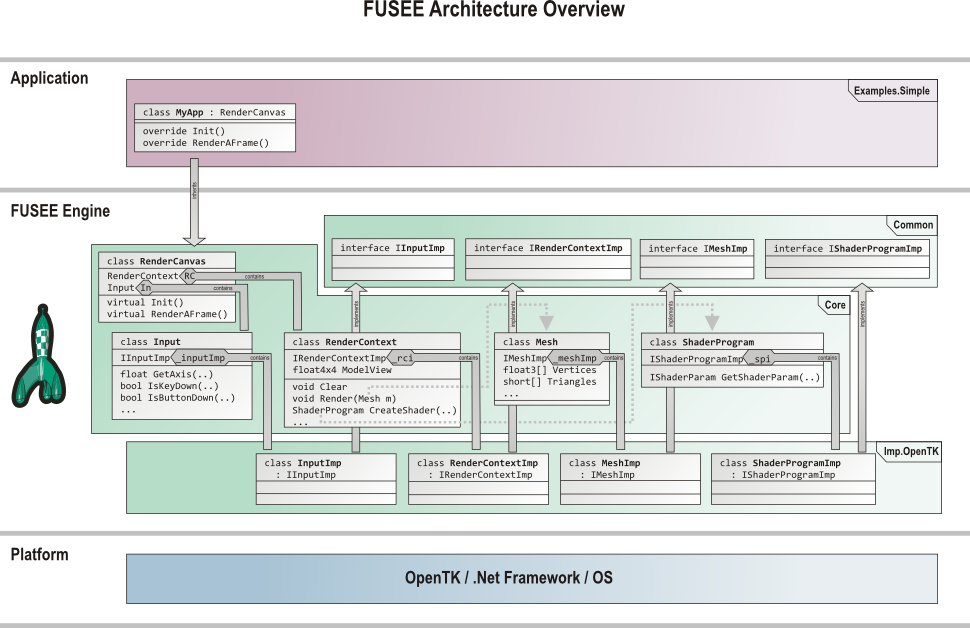
\includegraphics[width=0.8\textwidth]{images/FuseeArchitecture}
  }
  \caption{Fusee Aufbau}
  \label{fig:FuseeAufbau}
\end{figure}

Seinen modularen Aufbau erreicht Fusee dadurch, dass der Programmcode in drei Bereiche aufgeteilt wird. Der 'Core' beinhaltet alle grundlegenden internen Funktion, der 'Platform Adapter' beinhaltet die Anprogrammierung externen Codes und 'Common' stellt die Funktionalität der Implementierung über Interfaces bereit.

\subsection{CINEMA 4D}
\label{sec:c4d}

CINEMA 4D\footnote{http://www.maxon.de/} ist eine kostenpflichtige 3D-Grafiksoftware von der MAXON Computer GmbH. Sie wird seit 1990 entwickelt und ist mit ihrem aktuellen (2014) Update in Version R16 für Windows und Max OS X verfügbar. Mit CINEMA 4D unterstützt unter anderem Modellierung, Texturierung, Animation und eine Möglichkeit der grafischen Programmierung (XPresso).

Mit XPresso ist Node basiert, es ermöglicht also über Verbindungslinien Abhängigkeiten zwischen Objekten zu definieren. Zum Beispiel die Anzahl der Segmente des einen Objekts wird zur Position des anderen Objektes (Siehe \autoref{fig:C4D}). XPresso stellt alle relevanten Logik- und Rechenoperationen verfügbar um auch komplexere Probleme zu Lösen.
\begin{figure}[htbp]
  \centering
  \fbox{
    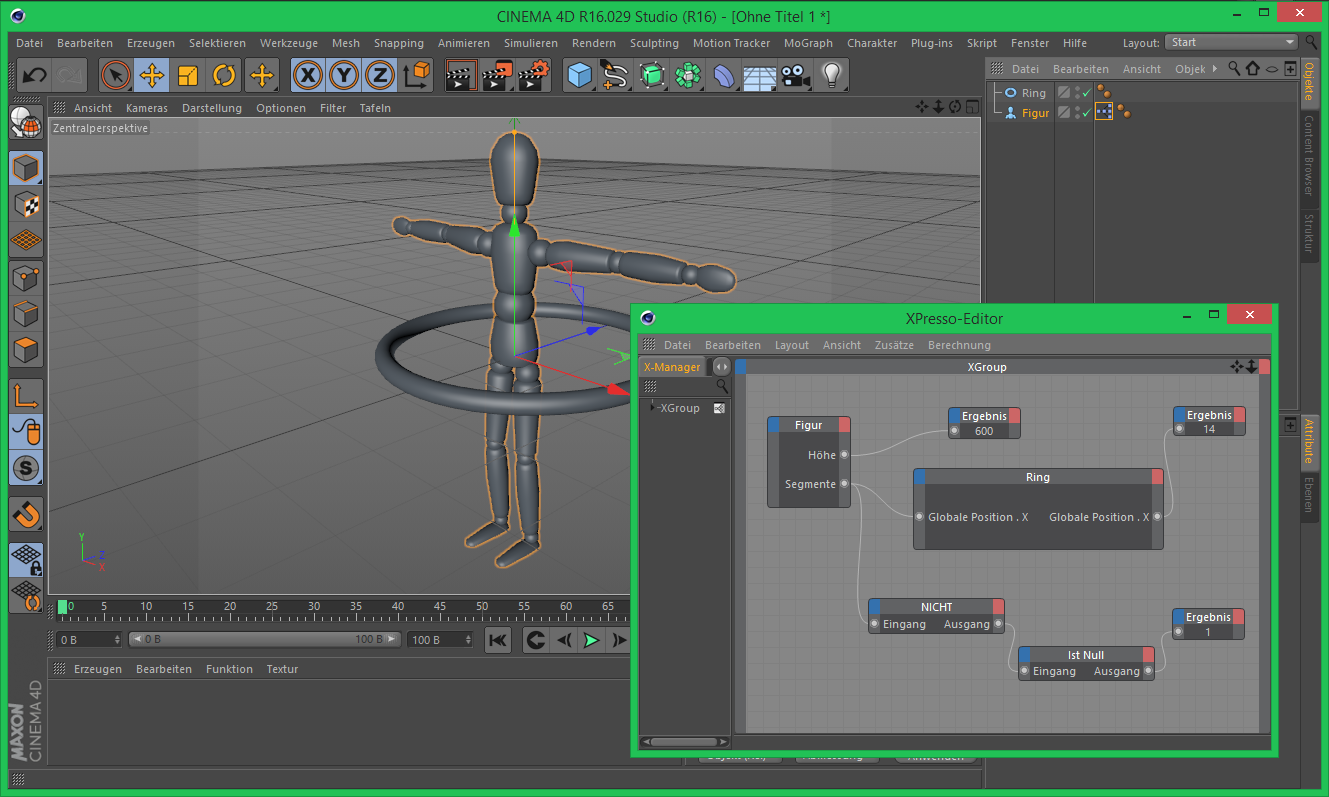
\includegraphics[width=0.8\textwidth]{images/C4D-1}
  }
  \caption{CINEMA 4D mit XPresso-Editor}
  \label{fig:C4D}
\end{figure}

\subsection{Unity}
\label{sec:unity}

Unity\footnote{http://www.unity3d.com/} ist eine 3D-Grafik-Engine die von Unity Technologies entwickelt wird und sowohl in einer Kostenlosen als auch Kostenpflichtigen-Version verfügbar ist. Unity besteht aus einer Laufzeitumgebung und einem grafischen Editor \cite{Gregory.2014}[S.29]. Im Editor können Objekte im 3D-Raum platziert werden oder er kann als Vorschau für die aktuelle Szene zur Laufzeit verwendet werden. Er ist nicht geeignet Objekte zu modellieren, dies geschieht in der Regel mit anderen Werkzeugen, zum Beispiel mit \nameref{sec:c4d}.
Unity ist Komponentenbasiert, das heißt, die Möglichkeiten ein von Objekten zu beinflussen werden dadurch verändert, dass eine Komponente dem Objekt hinzugefügt wird. Auf \autoref{fig:Unity} im rechten Teilfenster, dem \emph{Inspector}, ist zu sehen, dass dem Objekt \emph{Ship} eine \emph{Transform}-Komponente und eine \emph{Script}-Komponente vom Typ \emph{ShipScript} zugewiesen ist.

\begin{figure}[htbp]
  \centering
  \fbox{
    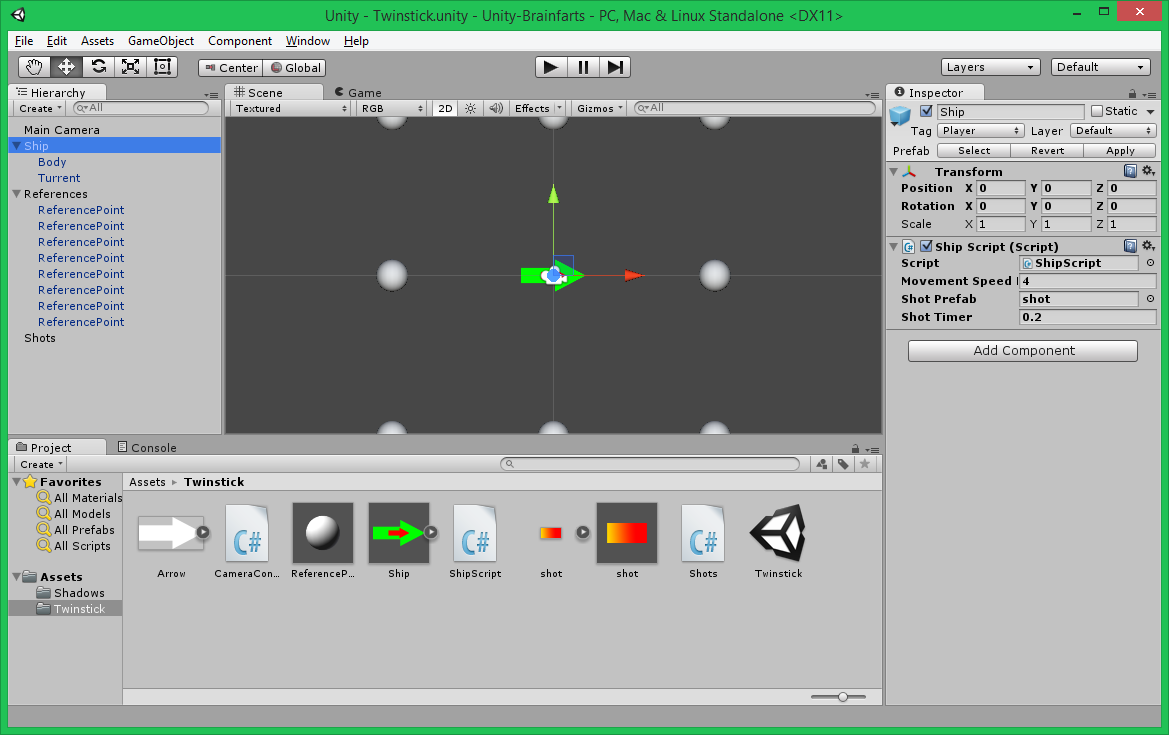
\includegraphics[width=0.8\textwidth]{images/Unity}
  }
  \caption{Unity Editor}
  \label{fig:Unity}
\end{figure}

\subsection{Open Game Engine Exchange (OpenGEX)}
\label{sec:OpenGEX}

MayBee Sumsumsum Kapitel